\begin{SCfigure}
    \centering
    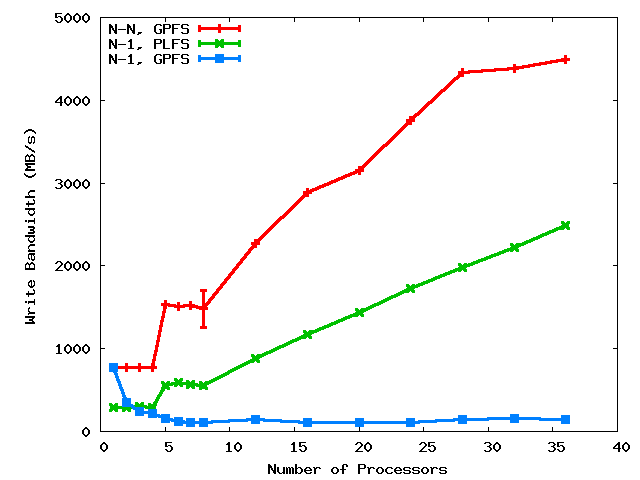
\includegraphics[width=0.4\textwidth]{data/overhead/gpfs.eps}
    \mycaption{fig-overhead}{Overhead.}{
        Ideally, N-1
        patterns written through \plfs\ would be able to 
        achieve the bandwidth available to an N-N pattern
        written directly to the \upfs.  However, 
        this graph shows that various overheads make this
        difficult.  Even though
        there is overhead, the important
        point is that \plfs\ still allows an N-1 pattern to
        be written much more quickly than if it was written
        directly to the \upfs. 
        \vspace{.5cm}
    }
\end{SCfigure}
